% 例 3：矩形 ABCD, AB=6, AD=10, 沿 AE 折叠使 D 落在 BC 上的 F
% A(0,6) B(0,0) C(10,0) D(10,6)? 这里 AD=10 是较长边，AB=6 短边
% 重新约定：A 左下、B 右下、C 右上、D 左上；AB=6 (底)，AD=10 (左侧)
% 不对，根据题目 AB=6 (一条边), AD=10 (邻边), D 折到 BC 上的 F
% 题目典型摆法：A(0,0), B(6,0), C(6,10), D(0,10), CD 边即从 D(0,10) 到 C(6,10)
% E 在 CD 上 → 设 CE=8/3, DE=10/3。F 在 BC 上, BF=8, FC=2
\documentclass[tikz,border=4pt]{standalone}
\usepackage{ctex}
\usepackage{amsmath}
\usetikzlibrary{calc, decorations.markings}
\begin{document}
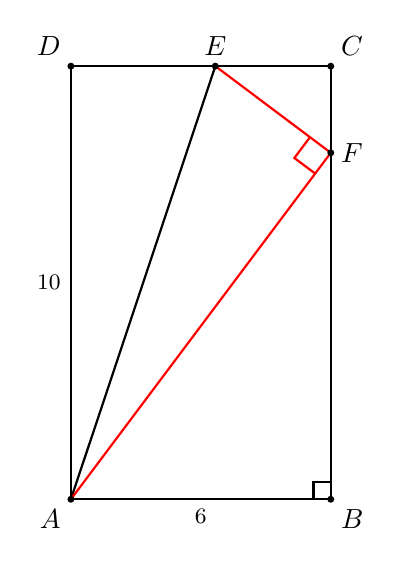
\begin{tikzpicture}[scale=0.55, thick]
  \coordinate (A) at (0,0);
  \coordinate (B) at (6,0);
  \coordinate (C) at (6,10);
  \coordinate (D) at (0,10);
  % BF = 8 → F = (6,8)
  \coordinate (F) at (6,8);
  % CE = 8/3, E 在 CD 上 (从 C 向 D): C + (8/3,0 along CD); CD 方向是 (-x)
  \coordinate (E) at ($(C)+(-8/3,0)$); % (6-8/3, 10) = (10/3, 10)
  \draw (A) -- (B) -- (C) -- (D) -- cycle;
  \draw (A) -- (E);
  \draw[red, thick] (A) -- (F);
  \draw[red, thick] (E) -- (F);
  % 标记直角 B
  \draw (6,0)++(-0.4,0) -- ++(0,0.4) -- ++(0.4,0);
  % 标记 ∠AFE = 90° (折叠像 ∠D)
  % AF 方向 (6,8)/10, FE 方向 (10/3-6, 10-8) = (-8/3, 2), 长度 sqrt(64/9+4) = sqrt(100/9) = 10/3
  % 简单画一个小方块
  \draw[red] ($(F)+(-0.36,-0.48)$) -- ($(F)+(-0.84,-0.12)$) -- ($(F)+(-0.48,0.36)$);
  \foreach \pt in {A,B,C,D,E,F} \filldraw (\pt) circle (1.5pt);
  \node[below left]  at (A) {$A$};
  \node[below right] at (B) {$B$};
  \node[above right] at (C) {$C$};
  \node[above left]  at (D) {$D$};
  \node[above]       at (E) {$E$};
  \node[right]       at (F) {$F$};
  % 标注尺寸
  \node[font=\footnotesize, below] at ($(A)!0.5!(B)$) {$6$};
  \node[font=\footnotesize, left]  at ($(A)!0.5!(D)$) {$10$};
\end{tikzpicture}
\end{document}
